% Created 2023-02-15 mer. 14:05
% Intended LaTeX compiler: pdflatex
\documentclass[presentation]{beamer}
\usepackage[utf8]{inputenc}
\usepackage[T1]{fontenc}
\usepackage[french]{babel}
\usepackage[labelformat=empty]{caption}
\usepackage{verbatim}
\definecolor{purple_wada}{RGB}{128,71,189} %   #8047bdff
\definecolor{links}{HTML}{2A1B81}
\useoutertheme{infolines}
%
% Beamer options
%
\setbeamertemplate{caption}{\raggedright\insertcaption\par}
\setbeamercovered{transparent}
\setbeamertemplate{section in toc}[sections numbered]
\setbeamertemplate{subsection in toc}[square]
\setbeamertemplate{navigation symbols}{}
\setbeamercolor{section in head/foot}{bg=purple_wada, fg=white}
\setbeamercolor{subsection in head/foot}{bg=white, fg=purple_wada}
\setbeamercolor{title in head/foot}{fg=purple_wada,bg=white}
\setbeamercolor{author in head/foot}{fg=white,bg=purple_wada}
\setbeamercolor{date in head/foot}{fg=white,bg=purple_wada}
\setbeamercolor{frametitle}{fg=purple_wada,bg=white}
\setbeamercolor{block title}{fg=purple_wada,bg=white}
%
% Adding frame at each section
%
\AtBeginSubsection[]
{
\begin{frame}
\frametitle{Sommaire}
\tableofcontents[currentsection,currentsubsection]
\end{frame}
}
\hypersetup{
colorlinks,
allcolors=.,
urlcolor=blue,
}
\usetheme{default}
\author{Doc. Malik Koné}
\date{28/01/2023}
\title{Transactions on blockchains}
\hypersetup{
 pdfauthor={Doc. Malik Koné},
 pdftitle={Transactions on blockchains},
 pdfkeywords={},
 pdfsubject={},
 pdfcreator={Emacs 28.2 (Org mode 9.4.6)}, 
 pdflang={French}}
\begin{document}

{
  \usebackgroundtemplate{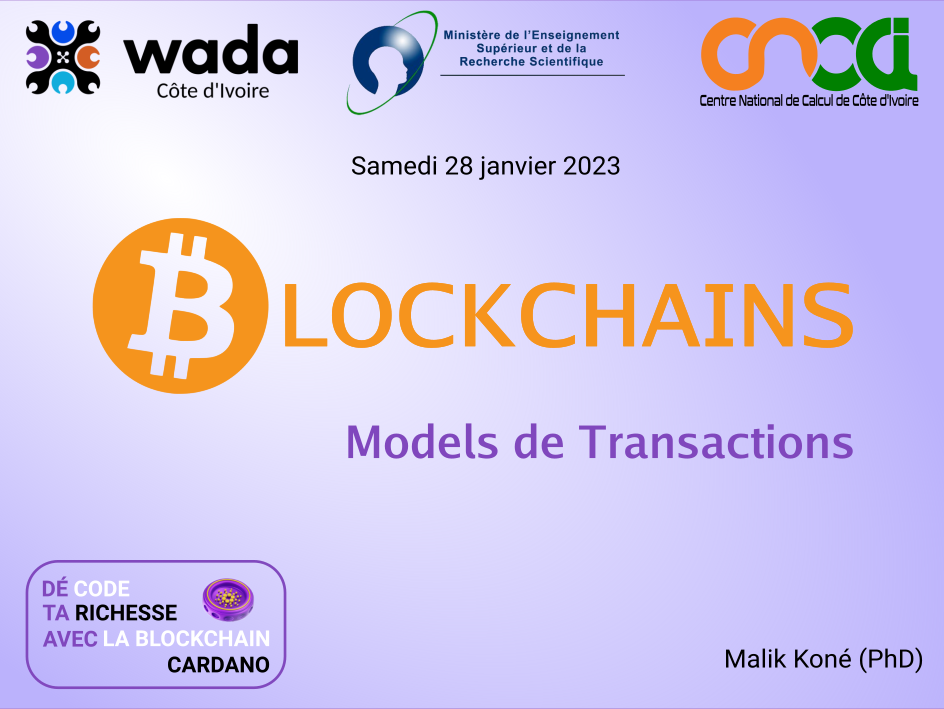
\includegraphics[height=\paperheight]{./page_de_garde_wadaci_j3a}}
  \frame[plain]{
  }
}

\section{Intro}
\label{sec:org48b280e}
\subsection{Les Cypher-punks}
\label{sec:orgd12e48a}
\begin{frame}[label={sec:orgb23d075}]{Les précurseurs du Bitcoin}
\begin{columns}
\begin{column}{0.6\columnwidth}
\begin{block}{}
\begin{itemize}
\item <1-> \href{https://en.bitcoinwiki.org/wiki/Hashcash}{Hashcash} (M. Back)
\item <2-> \href{https://nakamotoinstitute.org/secure-property-titles/}{Titres de propriété sécurisés}  (M. Szabo)
\begin{itemize}
\item Bit gold ; \emph{smart-contract}
\end{itemize}
\item <3-> \href{http://www.weidai.com/bmoney.txt}{B-money} (M. Dai)
\item <4-> Employé de PGP (M. Finney)
\begin{itemize}
\item 1er recipiendaire de BTC
\end{itemize}
\item <5> Voisin de Finney
\end{itemize}
\end{block}
\end{column}

\begin{column}{0.4\columnwidth}
\begin{block}<1->{}
\only<1>{

\begin{center}
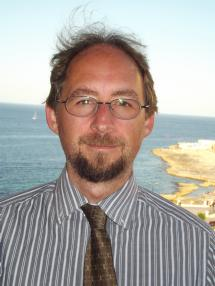
\includegraphics[width=.8\textwidth]{Images/adam.jpg}
\end{center}

}

\only<2>{
\begin{figure}[htbp]
\centering
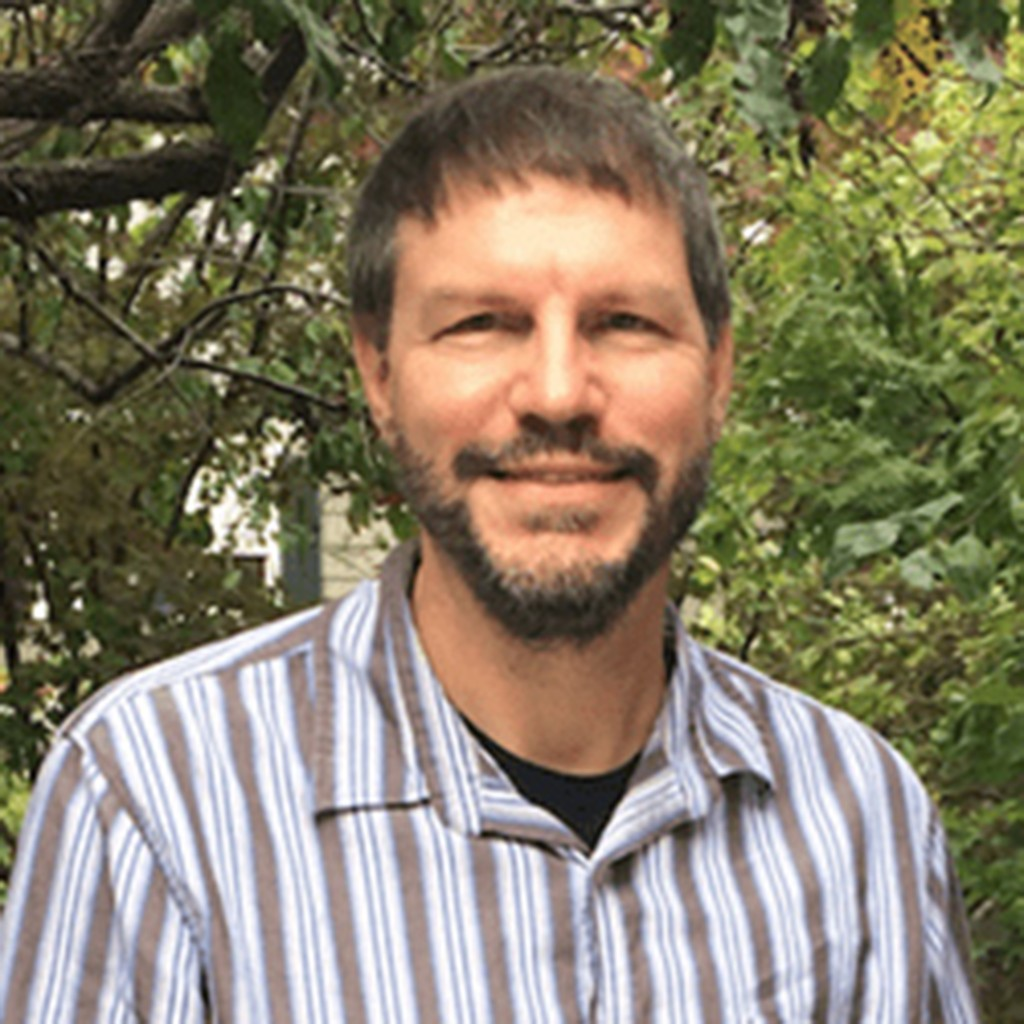
\includegraphics[width=\textwidth]{Images/nick_szabo.jpeg}
\caption{Nick Szabo}
\end{figure}

}
\only<3>{
\begin{figure}[htbp]
\centering
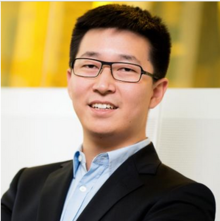
\includegraphics[width=\textwidth]{Images/wei_dai.png}
\caption{Wei Dai}
\end{figure}

}

\only<4>{
\begin{figure}[htbp]
\centering
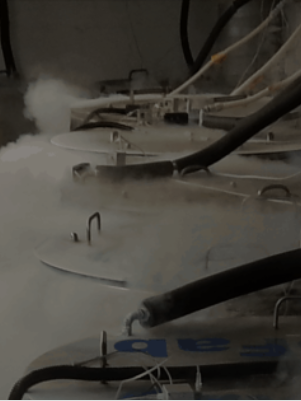
\includegraphics[width=.8\textwidth]{Images/hal_finney.png}
\caption{Hal Finney}
\end{figure}
}

\only<5>{
\begin{figure}[htbp]
\centering
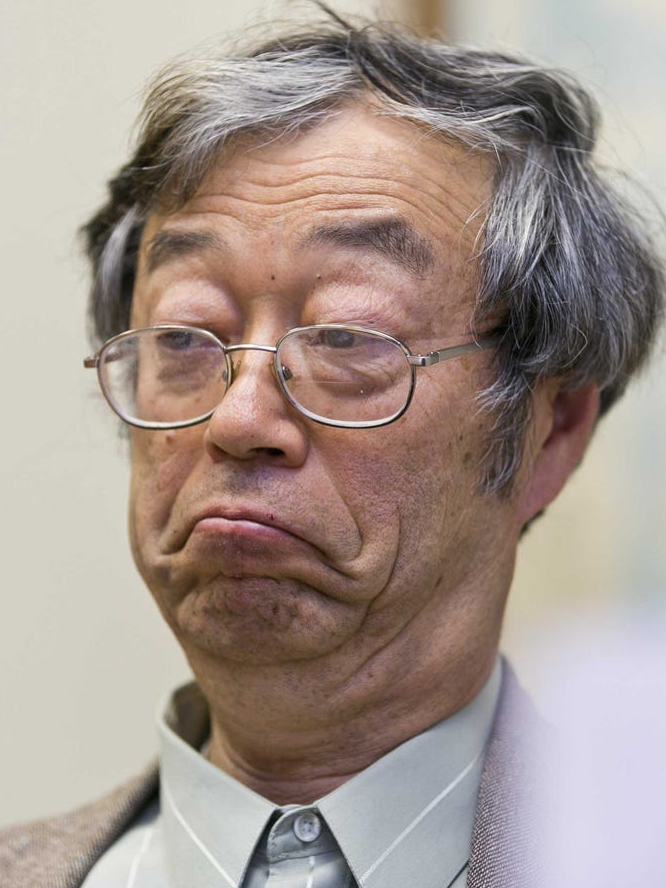
\includegraphics[width=.8\textwidth]{Images/dorian_nakamoto.png}
\caption{Dorian Nakamoto}
\end{figure}

}
\end{block}
\end{column}
\end{columns}
\end{frame}





\begin{frame}[label={sec:org504f219}]{Concept Cypher-punks}
\begin{itemize}
\item <1-> Un Escrow :  un garant, \alert{contrat de séquestre} (contrat de dépot)
\item <2-> Signature Elliptiques (ECDSA)
\begin{itemize}
\item Sécurité forte : de l'orde de \(2^{\text{longueur}(d_A)}\) ou \(d_A\) est la clef
\item Cryptographie asymétrique,  pair de clef (privée, public)
\item Utile pour signer les transactions
\end{itemize}
\item <3-> Merkle Tree :
\begin{itemize}
\item taille actuelle de la \href{https://ycharts.com/indicators/bitcoin\_blockchain\_size}{blockchain Bitcoin} : 450G
\end{itemize}
\item <4-> Fonction Hash160 = ripemd160(sha256(data))
\end{itemize}
\end{frame}

\begin{frame}[label={sec:org6ca5007}]{Futarchy : Voter les valeurs en pariant l'espérance}
\only<1>{
\begin{center}
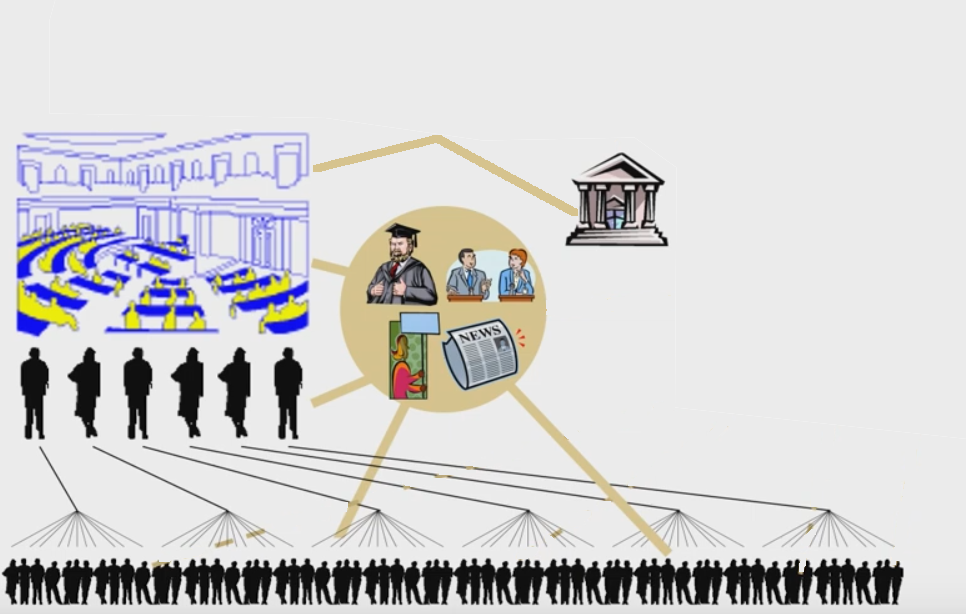
\includegraphics[height=.7\textheight]{Images/futarchy_depart.png}
\end{center}
}    

\only<2>{

\begin{center}
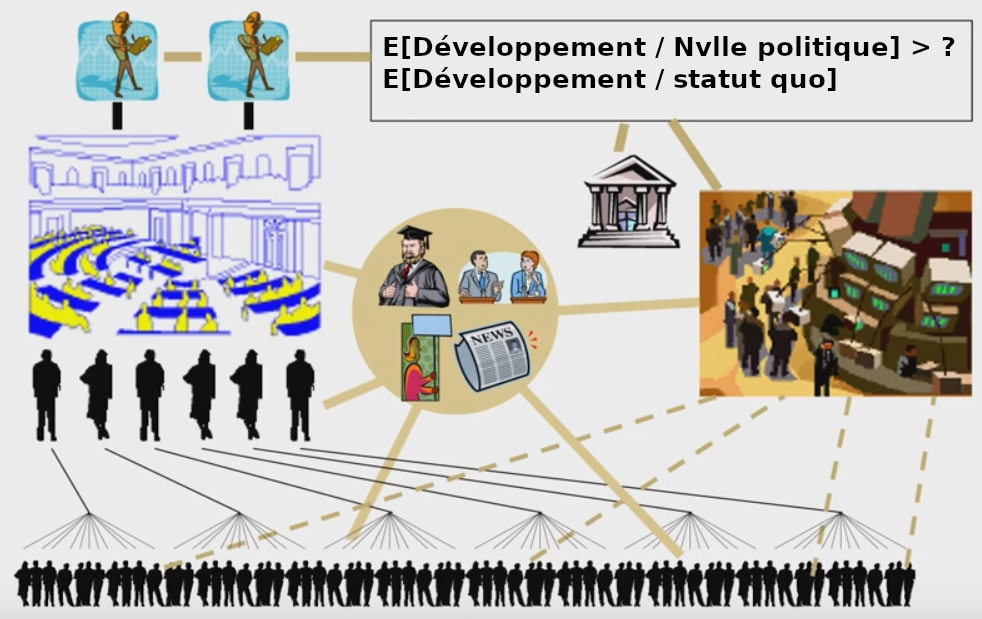
\includegraphics[height=.7\textheight]{Images/futarchy_all.png}
\end{center}


\begin{itemize}
\item Financiarisation des décisions politiques (\href{https://mason.gmu.edu/\~rhanson/futarchy.html}{Robin Hanson})
\end{itemize}


}    
\end{frame}

\section{Transactions Bitcoin}
\label{sec:org693f967}
\subsection{Transaction non dépensés uTXO}
\label{sec:orgb7b9c2a}
\begin{frame}[label={sec:org19312a9}]{Détaille d'un transaction non dépensée}
\begin{center}
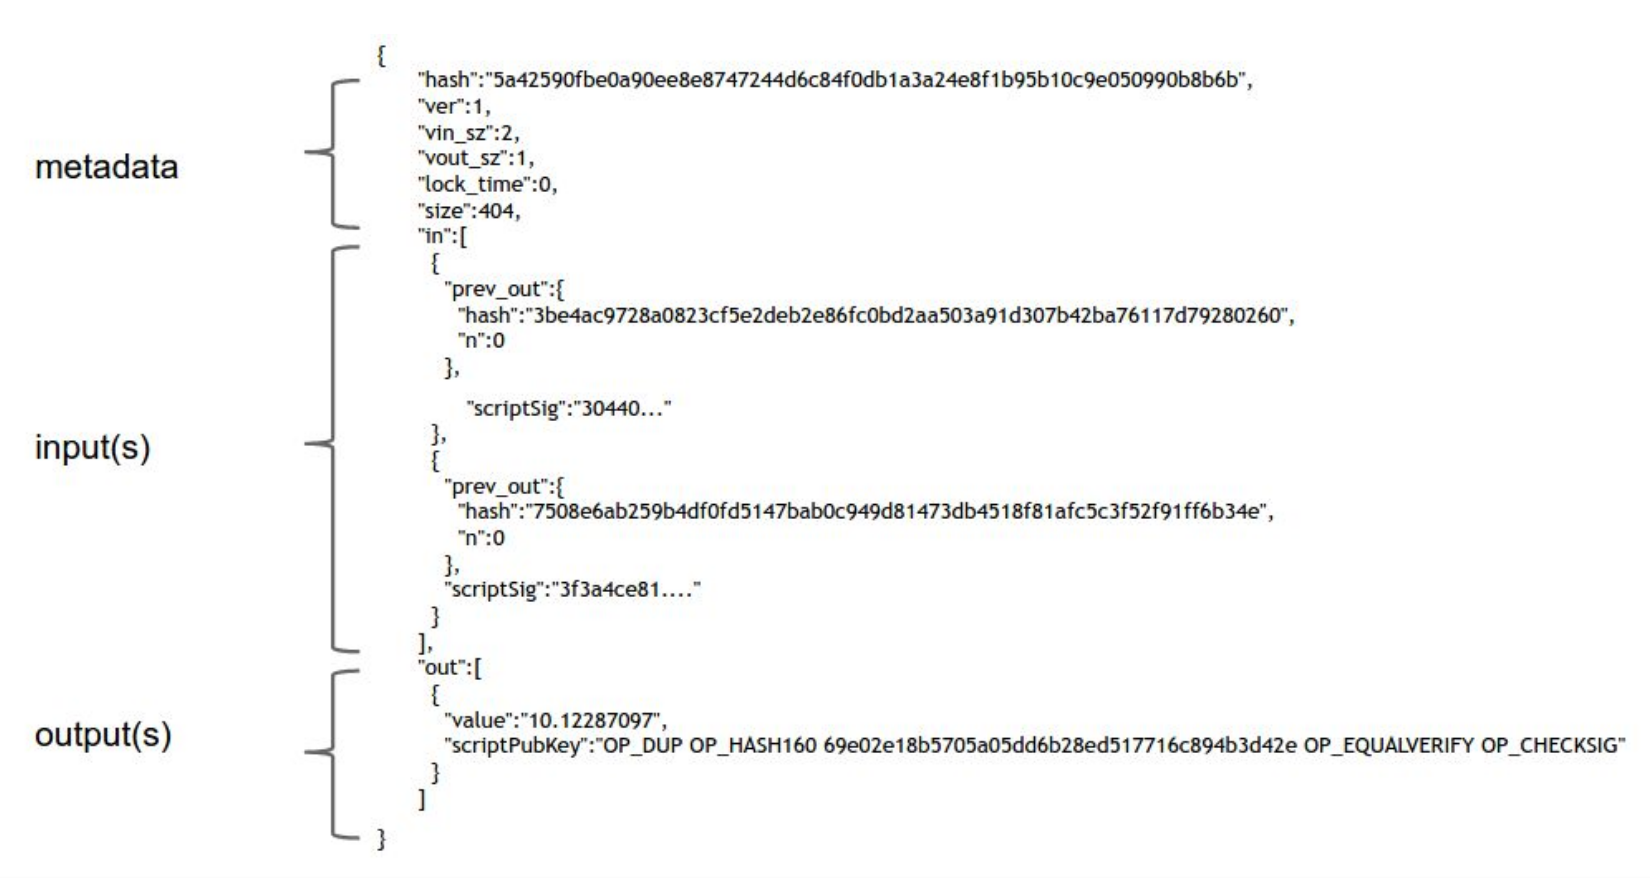
\includegraphics[width=.9\textwidth]{Images/transaction_btc.png}
\end{center}
\end{frame}
\subsection{Bitcoin Script}
\label{sec:org72d14df}
\begin{frame}[label={sec:org1132707}]{Un exemple}
\begin{columns}
\begin{column}{0.46\columnwidth}
\begin{block}<1->{Script "Payer à \ldots{} "}
\only<1>{
\begin{verbatiminput}
OP\_DUP\\
OP\_HASH160\\
69e02e18\ldots{}\\
OP\_EQAVLVERIFY\\
OP\_CHEKSIG
\end{verbatiminput}
}    

\only<2->{
\begin{verbatiminput}
<<sig>\\
<pubKey>\\

\noindent\rule{\textwidth}{0.5pt}
\end{verbatiminput}
\begin{verbatiminput}
OP\_DUP\\
OP\_HASH160\\
<pubKeyHash?>\\
OP\_EQAVLVERIFY\\
OP\_CHEKSIG\\
\end{verbatiminput}
}
\end{block}
\end{column}

\begin{column}{0.46\columnwidth}
\begin{block}<3>{Instructions}
\begin{itemize}
\item programmation en pile
\item 256 instructions 
\begin{itemize}
\item 15 désactivées
\item 75 réservées (pour plus tard)
\end{itemize}
\end{itemize}
(\href{https://en.bitcoin.it/wiki/Script}{liste complète sur en.bitcoin.it})
\end{block}
\end{column}
\end{columns}
\end{frame}
\begin{frame}[label={sec:orgbcfe472}]{Execution du Script "Payer à \ldots{}"}
\only<1>{
\begin{center}
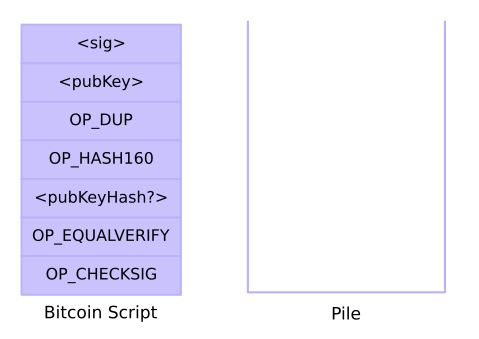
\includegraphics[height=.8\textheight]{Images/exec00.png}
\end{center}
 }

\only<2>{
\begin{center}
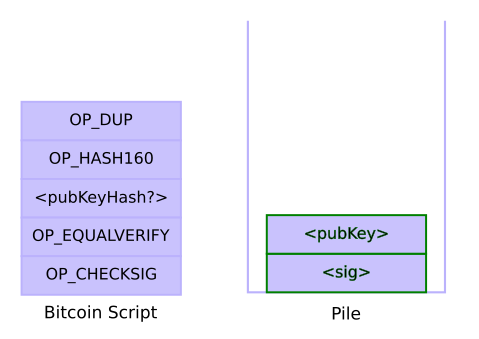
\includegraphics[height=.8\textheight]{Images/exec01.png}
\end{center}
 }

\only<3>{
\begin{center}
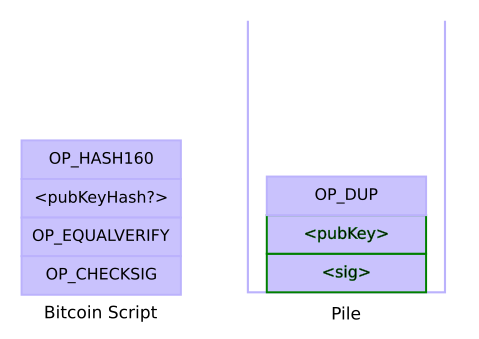
\includegraphics[height=.8\textheight]{Images/exec02.png}
\end{center}
 }

\only<4>{
\begin{center}
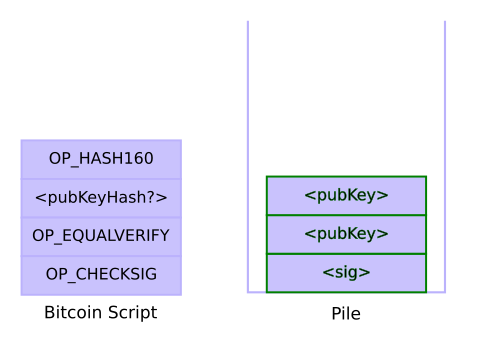
\includegraphics[height=.8\textheight]{Images/exec02b.png}
\end{center}
 }

\only<5>{
\begin{center}
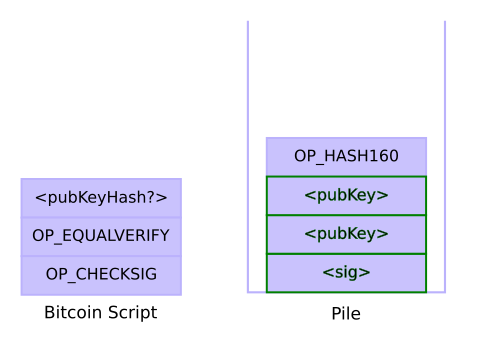
\includegraphics[height=.8\textheight]{Images/exec03.png}
\end{center}
 }

\only<6>{
\begin{center}
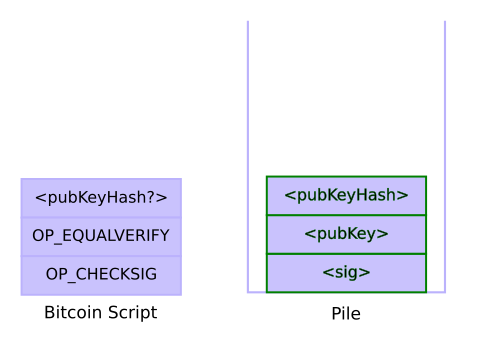
\includegraphics[height=.8\textheight]{Images/exec03b.png}
\end{center}
 }

\only<7>{
\begin{center}
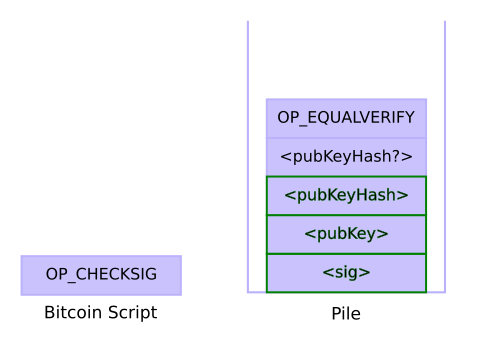
\includegraphics[height=.8\textheight]{Images/exec04.png}
\end{center}
 }

\only<8>{
\begin{center}
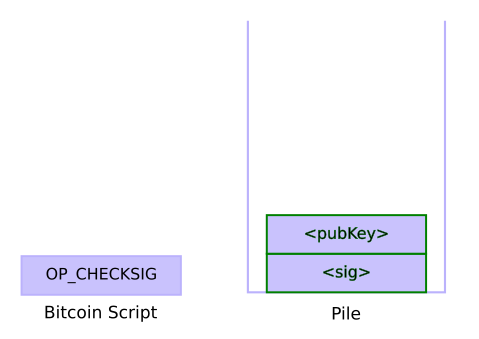
\includegraphics[height=.8\textheight]{Images/exec05.png}
\end{center}
 }

\only<9>{
\begin{center}
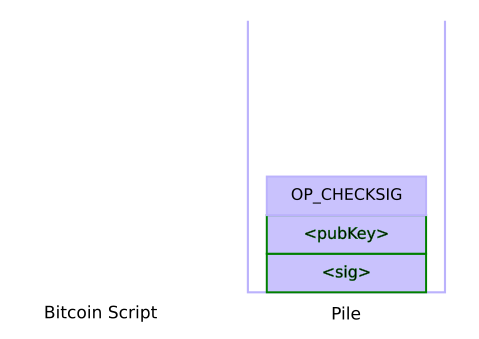
\includegraphics[height=.8\textheight]{Images/exec06.png}
\end{center}
 }

\only<10>{
\begin{center}
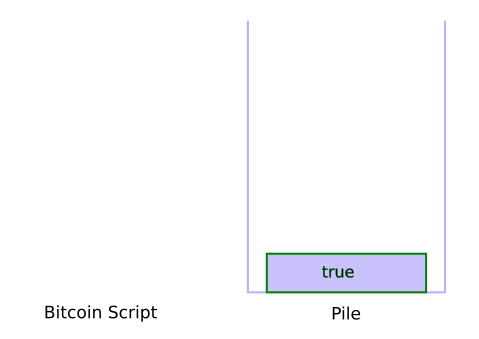
\includegraphics[height=.8\textheight]{Images/exec07.png}
\end{center}
 }
\end{frame}

\subsection{Les Limites du modèle Bitcoin}
\label{sec:org6357b14}
\begin{frame}[label={sec:org14f4857}]{}
\begin{itemize}
\item pas d'universalité
\item Ne connais pas la valeur de l'utxo
\item Une utxo est soit dépensée ou pas
\begin{itemize}
\item Il n'y a pas d'état intermédiaire
\end{itemize}
\item Le script n'a pas accès au nonce,  ni aux infos de la blockchain
\end{itemize}
\end{frame}
\section{Etherum}
\label{sec:orgac6a302}
\subsection{Avantages d'Etherum}
\label{sec:orgee46ec1}
\begin{frame}[label={sec:org1d82f65}]{Ce qu'Etherum apporte de nouveau}
\begin{itemize}
\item Accès à l'état de toute la blockchain
\item Permets des Applications (Universelles)
\item est moins énergivore (POW vs POS)
\end{itemize}
\end{frame}

\subsection{Similitudes Etherum - Bitcoin}
\label{sec:orgb4f058e}
\begin{frame}[label={sec:org5c1a322}]{Chaine de block}
\begin{center}
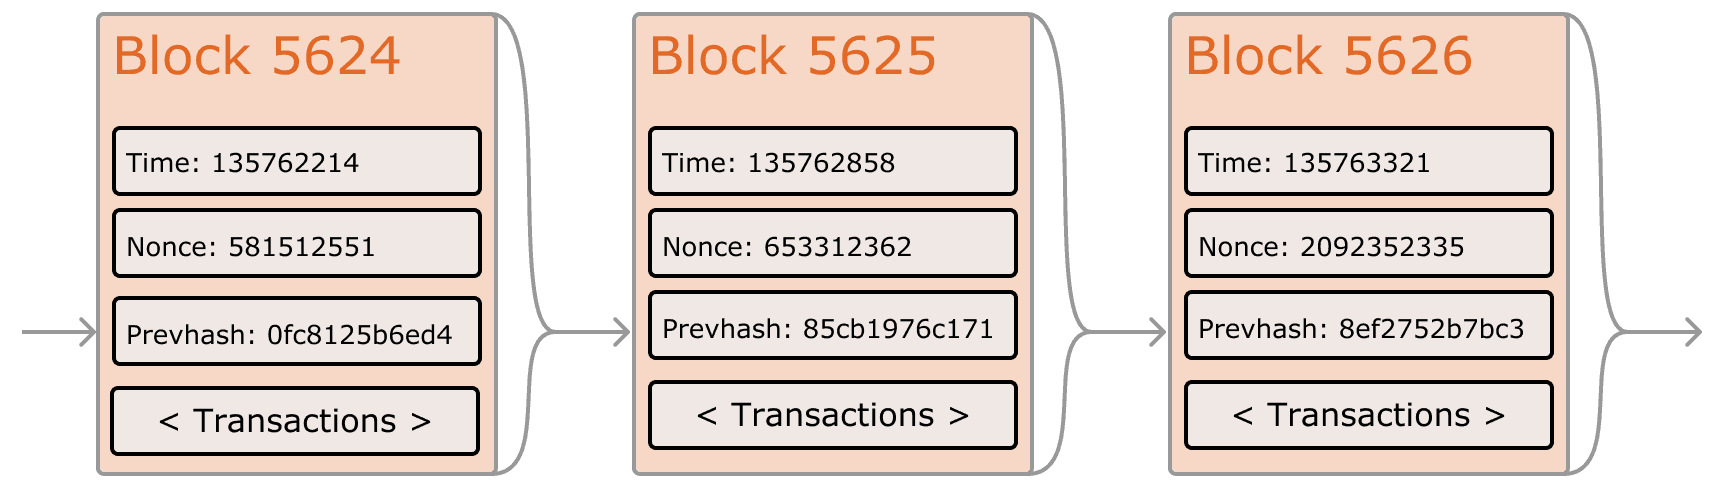
\includegraphics[width=\textwidth]{Images/ethereum-blocks.png}
\end{center}
\end{frame}
\begin{frame}[label={sec:org7e0a9e5}]{Arbre de Merkle}
\begin{center}
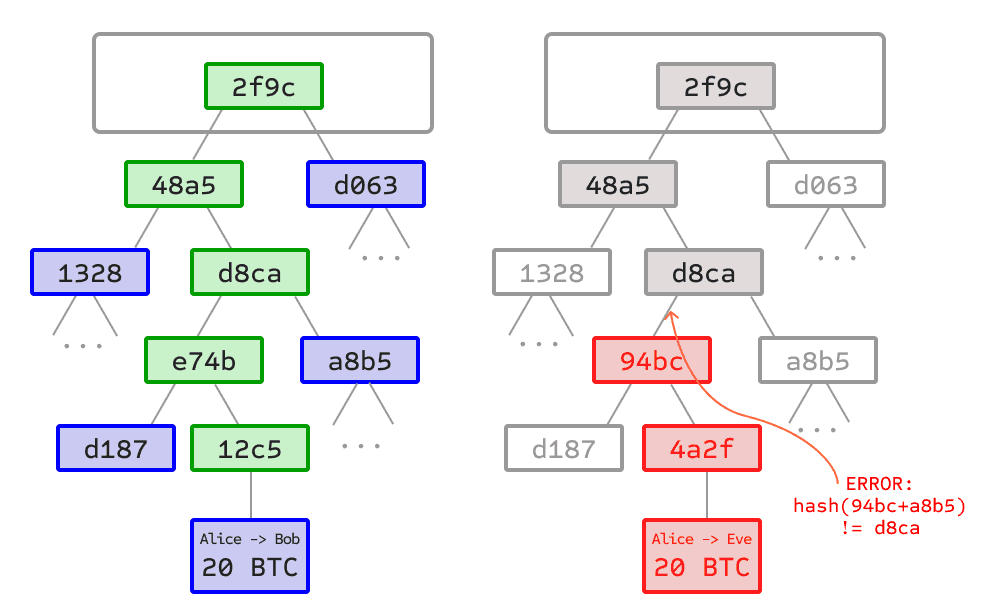
\includegraphics[width=.9\linewidth]{Images/spv-bitcoin.png}
\end{center}
\end{frame}

\begin{frame}[label={sec:org23151f8}]{Etats et transitions}
\only<1>{
\begin{center}
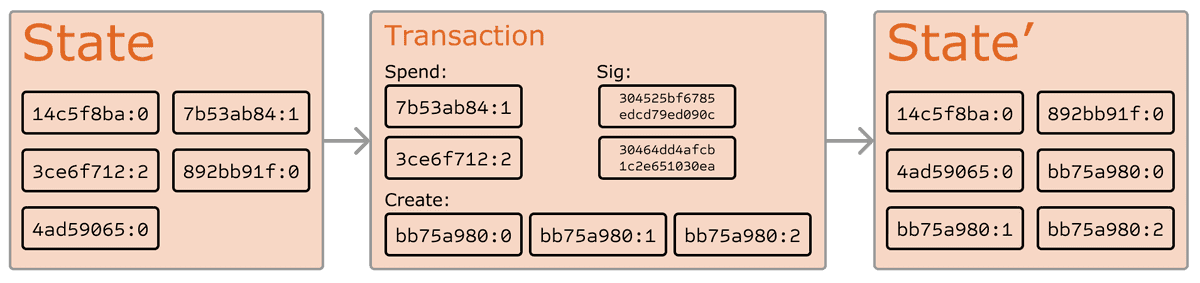
\includegraphics[width=\textwidth]{Images/ethereum-state-transition.png}
\end{center}
}

\only<2>{
\begin{center}
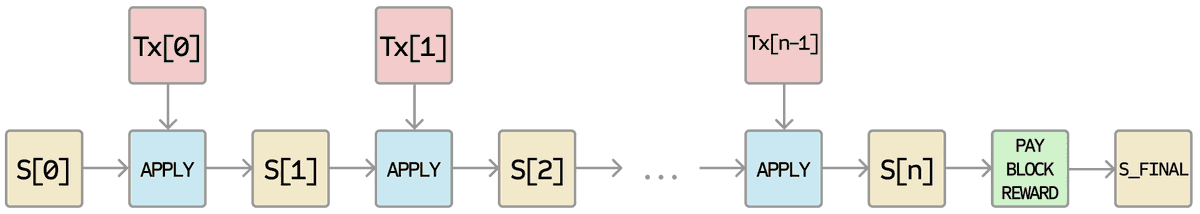
\includegraphics[width=\textwidth]{Images/ethereum-apply-block-diagram.png}
\end{center}

}
Les blockchain Etherum et Bitcoin peuvent être vue comme des systèmes à transition d'états
\end{frame}


\subsection{Différence Etherum - Bitcoin}
\label{sec:org2fcc8fd}
\begin{frame}[label={sec:orge74439f}]{Un autre modèle de transaction}
\begin{columns}
\begin{column}{0.5\columnwidth}
\begin{block}{}
\begin{block}{Compte Etherum}
\begin{itemize}
\item Nonce
\item Balance du compte
\item Code du contrat
\item <2> Espace de stockage
\begin{itemize}
\item stack : FIFO
\item memory : un tableau de taille variable
\item storage : pour le long terme
\end{itemize}
\end{itemize}
\end{block}
\end{block}
\end{column}

\begin{column}{0.5\columnwidth}
\begin{block}{}
\begin{figure}[htbp]
\centering
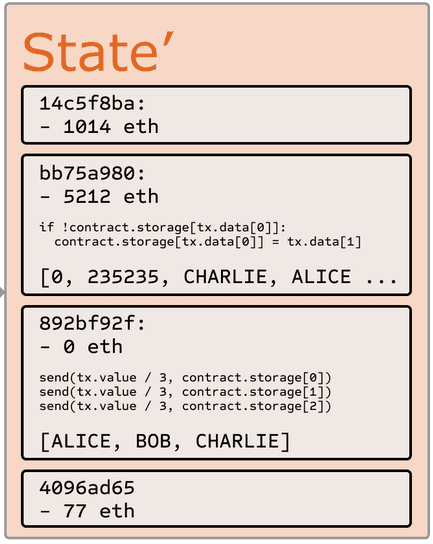
\includegraphics[width=.6\textwidth]{Images/etat_etherum.png}
\caption{Exemple d'un nouvel état}
\end{figure}
\end{block}
\end{column}
\end{columns}
\end{frame}

\begin{frame}[label={sec:org5296c83}]{Messages ou transactions Etherum}
\begin{block}{Ils peuvent}
\begin{itemize}
\item être crée \emph{on-chain}
\item contenir des données
\item être des réponses à un autre message
\item accéder à tout l'état de la blockchain
\end{itemize}
\end{block}
\end{frame}

\begin{frame}[label={sec:org84ae2f5},fragile]{Deux exemples de "smart contract"}
 \begin{block}{Remplace une donnée sur la blockchain}
\begin{verbatim}
if !contract.storage[msg.data[0]]:
   contract.storage[msg.data[0]] = msg.data[1]
\end{verbatim}
\end{block}

\begin{block}{Envois un montant à quelqu'un}
\begin{verbatim}
def send(to, val):
  if self.storage[msg.sender] >= val:
     self.storage[msg.sender] = self.storage[msg.sender] - val
     self.storage[to] = self.storage[to] + val
\end{verbatim}
\end{block}
\end{frame}

\subsection{Exécution d'un contrat}
\label{sec:orgb45a422}
\begin{frame}[label={sec:org90b16cd}]{Exécution d'un contrat}
\begin{block}{Objectif}
\begin{itemize}
\item Les frais sont limités par STARTGAS x GASPRICE
\item En cas d'erreur tout doit aller au mineur
\item En cas de réussite le mineur ne prend que ce qui a été consommé et le reste retourne au créateur de la transaction
\end{itemize}
\end{block}

\begin{block}{Plus précisement}
\begin{verbatiminput}
11: Vérifier le format de la transactoin\\
2: Prendre STARTGAS * GASPRICE dans balance de l'envoyeur\\
3: Enlève frais de la transaction dans les STARTGAS, 5 gas / byte\\
4: Fais le transfert de valeur\\
5: Fait tourner le code dans EVM\\
6: calcule combien de GAS on été dépensé et renvois le reste à l'envoyeur\\
\end{verbatiminput}
\end{block}
\end{frame}

\subsection{Applications}
\label{sec:org5f8c251}
\begin{frame}[label={sec:orgef83b21}]{Application purement financières}
\begin{columns}
\begin{column}{0.5\columnwidth}
\begin{block}{}
\begin{itemize}
\item Sous-monnaies
\begin{itemize}
\item stable coins
\end{itemize}
\item produits dérivés
\item contrat hedging
\begin{itemize}
\item assurances, \href{https://blog.ethereum.org/2014/03/28/schellingcoin-a-minimal-trust-universal-data-feed}{SchellingCoin}
\end{itemize}
\item Compte d'épargne
\item Application notariale
\item contrat de travail
\item loterie
\item marché distribués
\end{itemize}
\end{block}
\end{column}
\begin{column}{0.35\columnwidth}
\begin{block}{}
\begin{center}
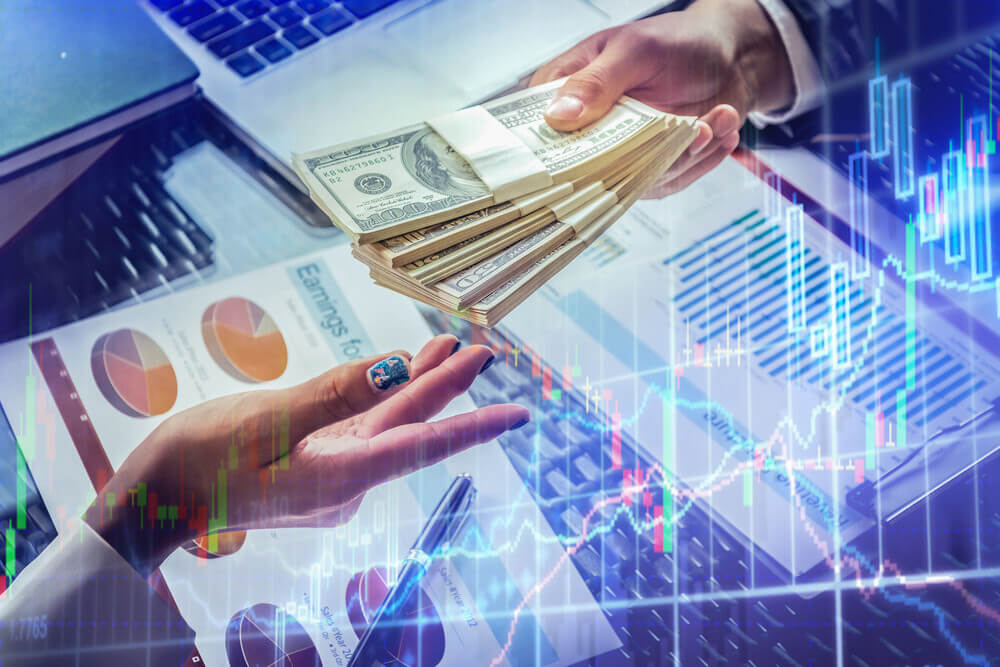
\includegraphics[width=\textwidth]{Images/defi_service.jpeg}
\end{center}
\end{block}
\end{column}
\end{columns}
\end{frame}

\begin{frame}[label={sec:org717bcc4}]{Applications semi-financières}
\begin{columns}
\begin{column}{0.49\columnwidth}
\begin{block}{Monnaies  et données}
Être payés pour, ou fournir, des données
\begin{block}{gestions des identités}
\begin{itemize}
\item gestion de nom de domaine (nameCoin)
\item gestoin d'ID
\item gestion de fichiers
\item gestion de contenu
\item réseau sociaux décentralisé
\end{itemize}
\end{block}
\end{block}
\end{column}
\begin{column}{0.45\columnwidth}
\begin{block}{}
\only<1>{
\begin{center}

\includegraphics[width=\textwidth]{Images/id_management.png}
\end{center}

}

\only<2>{

\alert{Autres Applications:}
\begin{itemize}
\item Calcul distribué\\
(seti@home, folding@home)
\end{itemize}

}
\end{block}
\end{column}
\end{columns}
\end{frame}

\begin{frame}[label={sec:org4ce75b9}]{Applications non-financières}
\begin{columns}
\begin{column}{0.35\columnwidth}
\begin{block}{}
\begin{itemize}
\item Vote en ligne
\item Gouvernance décentralisé
\end{itemize}
\end{block}
\end{column}
\begin{column}{0.5\columnwidth}
\begin{block}{}
\begin{center}
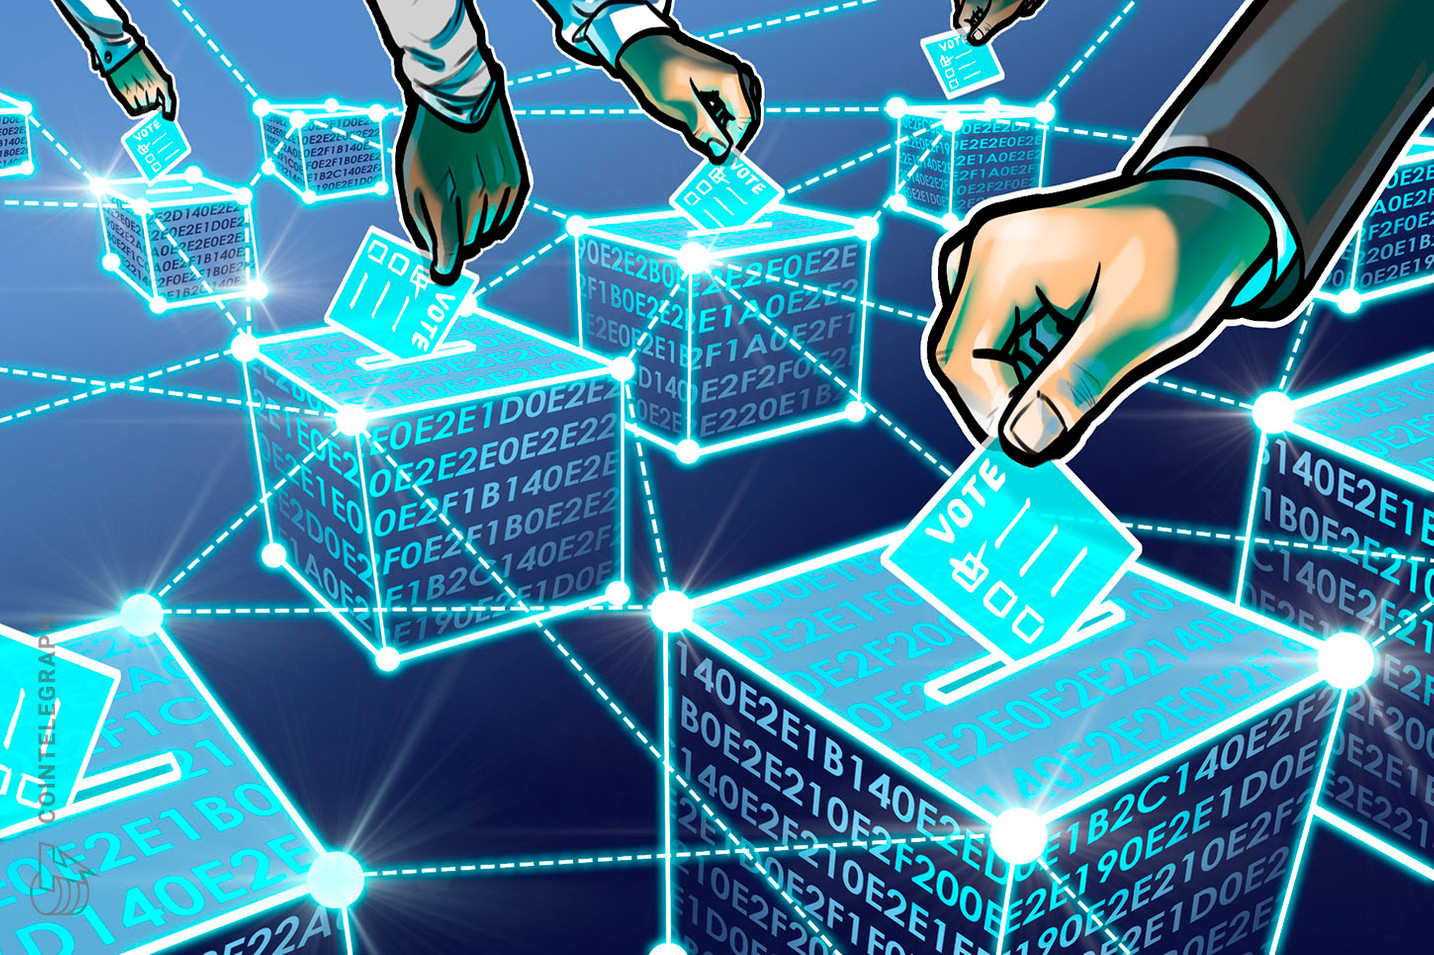
\includegraphics[width=\textwidth]{Images/block_vote.jpeg}
\end{center}     
\end{block}
\end{column}
\end{columns}
\end{frame}
\begin{frame}[label={sec:org8e1a89f}]{Applications Autonome et Décentralisé}
\begin{block}{DA : Decentralised Autonomous}
\begin{itemize}
\item DAC communauté (equal vote)
\end{itemize}
\begin{itemize}
\item DAC corporation (votre proportional to share)
\end{itemize}
\end{block}
\begin{block}{DAO : Decentralised Autonomous Organisation}
Peut fonctionner avec des individus ne parlant pas la même langue
\begin{itemize}
\item Automatise de la gouvernance
\end{itemize}
Code modifiable car stoqué dans la zone de stoquage des contrats
\begin{itemize}
\item modifié à l'aide de pointeurs
\end{itemize}
\end{block}
\end{frame}

\begin{frame}[label={sec:orgdfc7ef5}]{Divers}
\begin{itemize}
\item ICO: Initial coin offering
\item ASIC : Application speecific integrated circuits
\end{itemize}
\end{frame}


\section{Références}
\label{sec:org856e539}
\subsection{Références}
\label{sec:orgc35cef7}
\begin{frame}[label={sec:orgf2a873b}]{}
\begin{block}{Article fondateur des smart-contracts}
\begin{itemize}
\item Whitepaper d'Etherum (\href{https://ethereum.org/669c9e2e2027310b6b3cdce6e1c52962/Ethereum\_Whitepaper\_-\_Buterin\_2014.pdf}{pdf})
\end{itemize}
\end{block}

\begin{block}{CV de personnages celfs}
\begin{itemize}
\item \href{https://en.bitcoinwiki.org/wiki/Adam\_Back}{Adam Back} :  \href{https://www.youtube.com/watch?v=HEZAlNBJjA0}{vidéo}
\item \href{https://en.bitcoinwiki.org/wiki/Nick\_Szabo}{Nick Szabo} : \href{https://www.youtube.com/watch?v=tWuN2R2DC6c}{vidéo}
\item \href{https://en.bitcoinwiki.org/wiki/Wei\_Dai}{Wei Dai}
\end{itemize}
\end{block}
\begin{block}{Liens pour une introduction aux smart-contracts sur Cardano}
\begin{itemize}
\item \url{https://play.marlowe-finance.io}
\item \url{https://run.marlowe-finance.io/}
\end{itemize}
\end{block}
\end{frame}
\end{document}